\chapter{KopenVerkopen}\label{kvk}

"KopenVerkopen", which literally means "BuySell" in English, is an internal project started in early Summer 2015. It is supposed to be a mobile alternative to \href{http://www.marktplaats.nl/}{marktplaats.nl}, which is the Dutch equivalent to the French website \href{http://www.leboncoin.fr/}{leboncoin.fr}.

\medskip

Pierre and Matthias were working on that project mainly during their "spare time", which basically was either when their client projects were not late on schedule or when the clients were \textbf{not} putting them under pressure because of bugs, issues or enhancements -- which happened rarely. Consequently, that project was still in an early stage and not much progress had been made. As soon as my project Bearleaders was canceled, I was reoriented to KopenVerkopen.

\section{Why an internal project}

The original idea behind that mobile application was the show to potential clients what the Smiths was able to do. As a development agency, we have a portfolio\footnote{\href{http://www.wearesmiths.com/}{www.wearesmiths.com}} listing all the projects we had been working on. Thus, they thought it would be a great thing to add a home-made app on it, just to show off.

\medskip

In the meantime, Pierre and Matthias saw that as the opportunity to try new technologies or libraries, so that we would improve our skills with no risk as the client was... us. Just like a playground, it was meant to carry out experiments of any type with Titanium as well as experiments in mobile development in general.

\section{What it is}

KopenVerkopen is, as I said, a selling app, for individuals. The concept is pretty simple: anyone can download the app and then easily log in using their Facebook account. Then, the user can either browse through items for sale or sell one of their items. The feed of items on sale can be filtered using different filters, like sorting from the closest buyer to the farthest one, according to the GPS location.

\medskip

When showing interest for an item on sale, the interested person is added to a stack of potential buyers. The owner of the product is then introduced to the first person of this list thanks to a conversation popping up on their screens, in a specific section of the app. The two people can now discuss about the sale itself. At any time, one of them can cancel the sale, which would remove the potential buyer from the list of interested people. In such a case, the owner would be introduced to the next potential buyer thereafter.

Finally, when both parties agreed on the sale, the owner can mark the item as "sold".

\medskip

Users can also manage their profile with a few basic options. The profile picture is the same one as on their Facebook profile. Furthermore, on the profile page, several shortcuts are available (see the figure \ref{tabs-kvk} right below).

\begin{figure}[H]
   \centering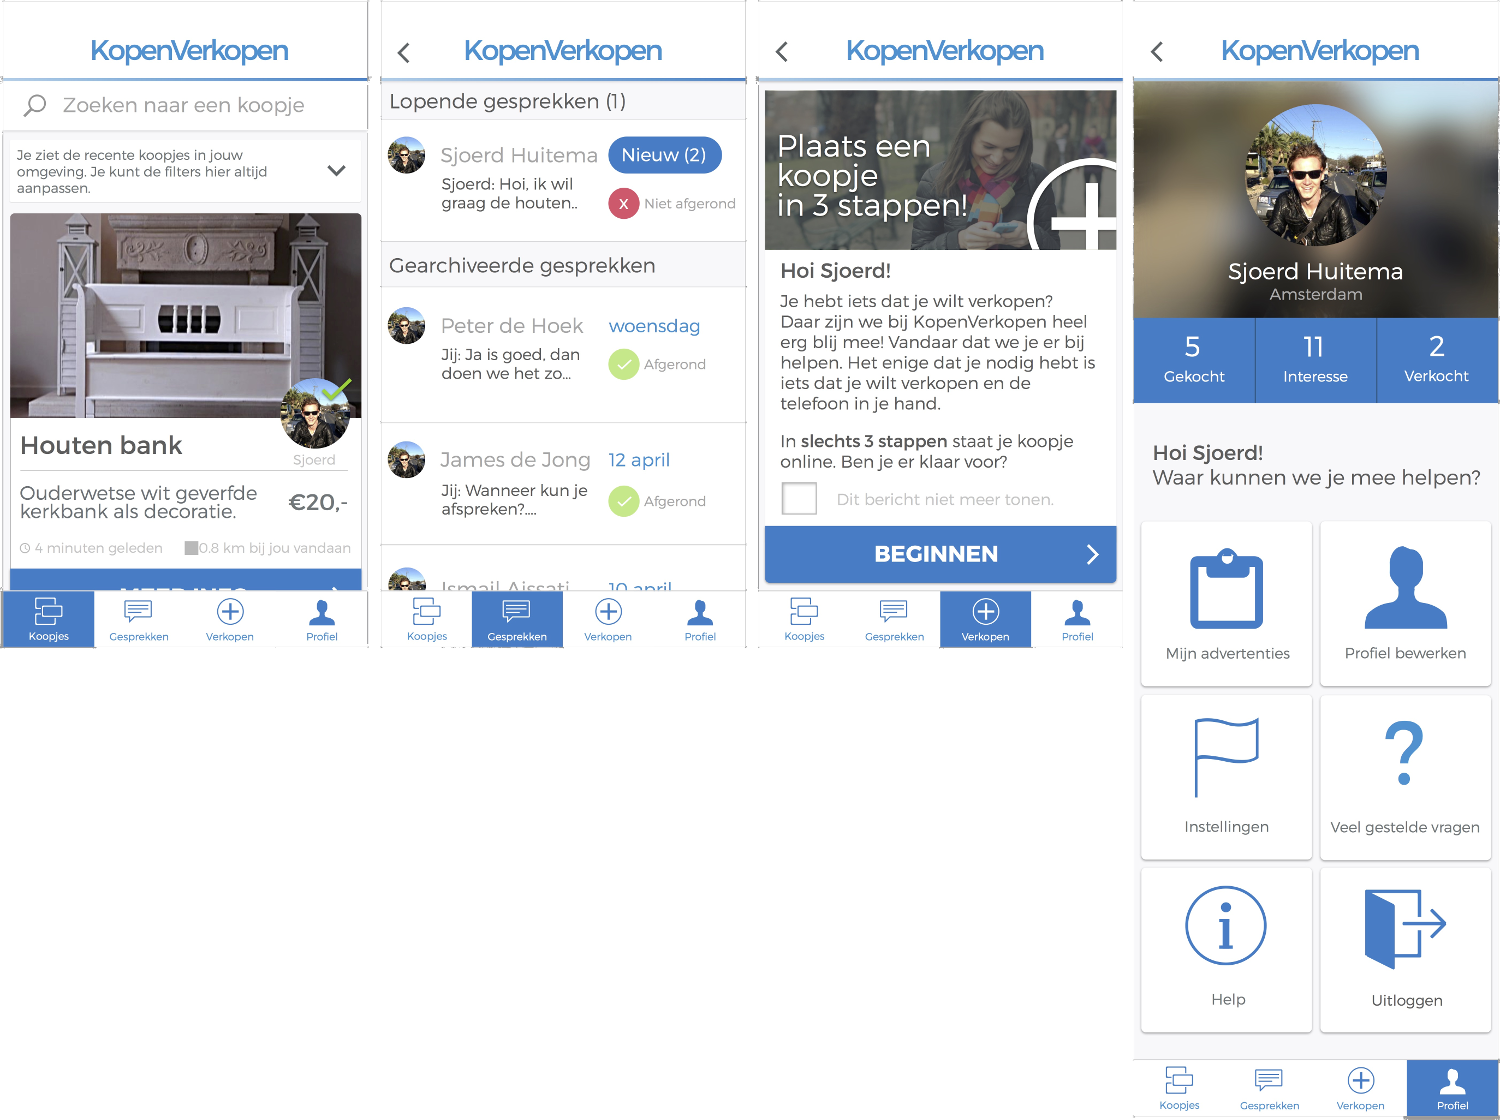
\includegraphics[width=1.00\textwidth]{images/kvk-tabs.png}
   \caption[The four main tabs of KopenVerkopen]{The four main tabs of KopenVerkopen\\From left to right: Feed of items on sale, Conversations with buyers/owner, Sell a new item, Profile and options}\label{tabs-kvk}
\end{figure}

\section{Road map, Strategy \& Reality}

The road map which seemed to be the most doable and realistic is as follows:

\begin{enumerate}
  \item Choosing carefully which features are relevant and needed (everyone)
  \item Designing the app (Matthias and the designer, Wessel)
  \item Writing the specifications formally (plus designing the UI\footnote{\textit{User Interface}})
  \item Coding (this part is a big one, hiding many sub-parts and iterations)
  \item Publishing
\end{enumerate}

\medskip

In parallel of the step 4, a lot of refactoring would be done on a regular basis, as well as code review sessions. Code reviews are meant to make sure everyone is heading in the right direction, and also to improve someone's code so that this person can learn from others. On the other hand, the goal of refactoring is to keep "innovating", improving our code, getting ride of obsolete code, and so forth.

\medskip

This schedule is somewhat simple and yet commonly encountered among software development. Nothing too much, as it would be an internal and experimental project. The allocated time was quite unsure, as we foresaw a lot of refactoring. Moreover, we would only work on that project during our "spare time", when client projects would wind down.

\medskip

When I arrived, back in September, the three first steps had almost already been conducted. The team was still polishing a bit the architecture, from time to time. Actually, the project had almost been paused. As of late October, it suddenly resumed, mostly because Bearleaders had been discontinued.

\medskip

During the first week "post-Bearleaders", I familiarized myself with the project, discovering its architecture, finding out what has been done so far, what was left to be done, and so forth. The specifications were available on our GitHub repository, mockups had also been created by Wessel. Soon enough, I noticed some issues in the current API and database\footnote{Parse.com does not provide a real database in the usual sense of the word. Instead, it is an abstraction of the underlying used MongoDB. But yet, developers -- us -- have to create sorts of simplified tables with typed columns. There are no triggers, no stored procedures, no constraints (not event \lstinline{PRIMARY KEY}, the system creates automatically a primary key for each row, with no possibility of deletion): all of them have to be written in specific files called "hooks", which are run before or after insertions automatically.}. I started to discuss it with Matthias and, as it often happens after a long period of inactivity, we were all agreed that there were few glitches that needed to be fixed. That was when we decided to go back to step 2. We did not need to edit the specifications as our changes would not have any effect on the mobile app itself.

\section{Involvement}

\subsection{API}

For approximately one or two weeks, I reused most of my blog post\footcite[See the reference][in the bibliography]{api_my_blog} about APIs to rethink ours. Matthias and I actually bought a set of whiteboard sheets to build a huge (4-meter long x 2 meters) whiteboard next to our desks, on a wall. We used it to write down our database structure as well as our API endpoints, linked to actions performable by users in the app. After this brainstorming period, he reflected all the changes to the back-end code and I did the same for the mobile app code.

\subsection{Example of a widget: ts.chat2}

In the meantime, I also updated a widget I had started in September, called "ts.chat2" which in turn is an upgraded version of "ts.chat".\\
"ts.chat" was a quite simple chat widget developed by Matthias which provided a minimalist -- though working like a charm -- UI for text messages, just like any SMS app. However, his widget used two modules to bring more features which turned out to be a problem: they were not very up-to-date and they introduced issues with newer versions of Titanium. I decided to get rid of those dependencies and develop a new widget, directly inspired from Matthias' one. It was also a great opportunity to explore widgets and their capabilities. As a reminder, widgets bring modularity which is a true strength of Titanium.

\begin{figure}[H]
   \centering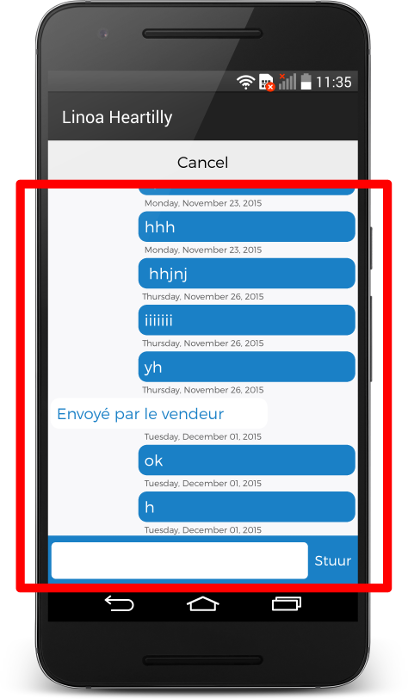
\includegraphics[width=0.45\textwidth]{images/tschat2framed.png}
   \caption[KopenVerkopen -- ts.chat2]{The red square shows the widget, included in a window}\label{tschat2pic}
\end{figure}

The widget receives a Backbone collection\footnote{\href{http://backbonejs.org/\#Collection}{http://backbonejs.org/\#Collection}} containing messages. It iterates through them in order to display them, from the oldest (on top of the screen) to the most recent. It also offers an input text field so that the user can add messages.

\medskip

The widget can trigger two distinct Backbone events:

\begin{enumerate}
  \item \lstinline{moremessages}: when the user scrolls to the very top of the screen
  \item \lstinline{newmessage} when the user has typed a message and sent it
\end{enumerate}

The first event is intended to fetch more messages from the server (older messages). The second one basically says that a new message is about to be sent (it also provides the message as a second argument, see the last line below):

\javascript
\begin{lstlisting}
var newmessageEvent = {
    message: $.typingArea.value,
    created_at: new Date(),
    success: function () {
        $.typingArea.value = "";
        _resizeTypingArea();
        $.sendBtn.touchEnabled = true;
        scrollToBottom();
    },
    error: function () {
        $.sendBtn.touchEnabled = true;
    }
};
$.trigger('newmessage', newmessageEvent);
\end{lstlisting}
Nevertheless, it is the responsibility of the developer to take care of that message.

\medskip

This widget works thanks to \textbf{data-binding}, a powerful concept, prominent within Titanium and deeply built-in\footnote{\href{http://docs.appcelerator.com/platform/latest/\#!/guide/Alloy_Data_Binding}{http://docs.appcelerator.com/platform/latest/\#!/guide/Alloy\_Data\_Binding}}. Basically, it is like linking a model or a collection of models (here \lstinline{Message}) to a view. As a result, the view would get automatically updated as soon as the model would change.

\medskip

In addition to the inner mechanism to handle messages, the widget offers some kind of customization. When included in a window, a few colors can be specified, for instance:

\begin{lstlisting}
$.chat.init({
    // Alloy.CFG.COLORS.x are defined in a global conf file
    messages: Alloy.Collections.messages, // The collection to use for Data Binding
    backgroundColor: Alloy.CFG.COLORS.WHITE_DARK,
    backgroundColorLeft: Alloy.CFG.COLORS.WHITE,
    colorLeft: Alloy.CFG.COLORS.BLUE,
    ...
    sendButton: { // Configuration for the button at the bottom right
        title: 'Stuur',
        borderRadius: 5,
        ...
    },
    typingArea: { // Configuration for the input text
        color: Alloy.CFG.COLORS.BLUE,
        ...
    },
    ...
});
\end{lstlisting}

\subsection{Entire app}

I got involved in other widgets (ts.prettymenu\footnote{\href{https://github.com/TheSmiths-Widgets/ts.prettymenu}{https://github.com/TheSmiths-Widgets/ts.prettymenu}}, ts.camera\footnote{\href{https://github.com/TheSmiths-Widgets/ts.camera}{https://github.com/TheSmiths-Widgets/ts.camera}}, and others not publicly available), but not as much as with \textit{ts.chat2}. Consequently, I will not detail them in this report.

\medskip

In summary, in chronological order, I have worked on:
\begin{itemize}
  \item \textbf{The conversations}: creating a new widget, updating the UI, inserting the widget, making sure it was working flawlessly.
  \item \textbf{Translations}: the app has been designed to support three languages (Dutch, English and French). I helped to translate some parts of the app.
  \item \textbf{Refactoring}: after the big decisions we had made regarding the back-end (API and data tables), new models had to be created based on the old ones. It also implied migrating the local databases (SQLite is used as a database for apps in both Android and iOS).
  \item \textbf{Polishing the UI}: conversations were reshaped many times to fit at best Wessel's design
  \item \textbf{Adding features to conversations}: I added a handful of features to the app, like two buttons to either cancel or sell an item
  \item \textbf{Bug fixing}: particularly in the dashboard (for some reason the menu was pretty bugged)
  \item \textbf{Adding features to the app}: logout, popups at different points (I had to create a widget for it by the way, see the figure \ref{popup} below), sharing capacities (on social media)
  \item \textbf{Bug fixing}: mainly on iOS, as I was developing on Android first
\end{itemize}
\begin{wrapfigure}{r}{0.4\textwidth}
  \vspace{-10pt} % hack
  \begin{center}
    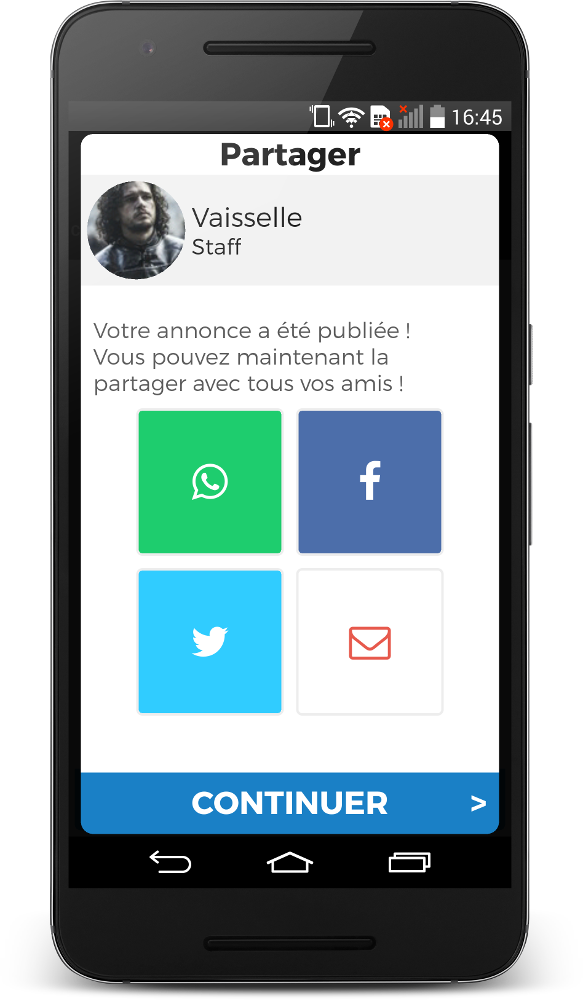
\includegraphics[width=0.35\textwidth]{images/popupframed.png}
  \end{center}
  \caption[KopenVerkopen -- Popup]{The popup showing social media icons}\label{popup}
  \vspace{-60pt} % hack
\end{wrapfigure}

In total, I had been spending roughly one week in September, and a whole month (from November, \nth{6} to December, \nth{9}).

\section{Current state and outcome}

As of early December, the project has been paused because of a new client project (see chapter \ref{tesco}). The back-end is fully operational and still running. The app is almost done. Most of the features have been implemented, a few ones excepted. However, there is still a lot of polishing to do and several glitches to fix. Although the app is in an advanced state, I would say that a bunch of months (perhaps two or three, tops) are yet to be spent working, on condition that two developers would work on it at least.

\section{Conclusion}

This project was really interesting as I had quite a lot of responsibilities, or a least the freedom to take decisions. Since it was an internal project, no money nor reputation was at stake. It was truly a deep-dive into Titanium. I really had the time to get a full overview of the entire framework (its advantages and drawbacks). In the meantime, it was a chance for me to contribute to the community by giving away widgets I had developed, or merely improving existing ones.

\medskip

After such an intense period dedicated to Titanium, I was able to weight the pros and cons regarding cross-platform mobile development, and more precisely Titanium. I had started to adopt techniques and best practices used by my colleagues to maintain a homogeneous code. More and more, I was feeling confident with JavaScript. That was somehow the pinnacle of my internship as I was gaining more experience everyday and learning from my colleagues efficiently. Our workflow had proven to be useful, it was bringing daily efficiency.